\section{\texorpdfstring{Adresace paměti}{Adresace pameti}}

% =====================================================================================================================
	\begin{frame}
    \frametitle{Adresace paměti instrukcí}
		\small
		
		\begin{itemize}
			\item \textbf{Každá instrukce určitým způsobem pracuje s pamětí:}
			
			\begin{enumerate}
				\item načtení hodnoty z paměti,
				\item provedení operace s načtenou hodnotou,
				\item uložení výsledku zpět do paměti.
			\end{enumerate}
			
			\vspace{1mm}
			\item \textbf{Zdrojovou nebo cílovou pamětí může být v případě procesorů STM8 jakákoliv paměť v jednotném adresním prostoru:}
			
			\begin{itemize}
				\item RAM,
				\item ROM,
				\item zásobník (STACK) -  zásobníkové adresování, ...
			\end{itemize}
			
			\vspace{1mm}
			\item \textbf{Existuje více možností jak instrukce předává adresu paměti:}
			
			\begin{itemize}
				\item implicitní (inherentní) adresování - instrukce bez operandů,
				\item bezprostřední adresování,
				\item přímé adresování,
				\item indexové adresování,
				\item nepřímé adresování,
				\item relativní adresování - skoky.
			\end{itemize}
		\end{itemize}

	\end{frame}
	
% =====================================================================================================================
	\begin{frame}
    \frametitle{Implicitní adresování}
		
		
		\begin{itemize}
			\item Instrukce nevykonává operaci s pamětí - nemá operandy,
			
			\vspace{2mm}
			\item strojový kód plně specifikuje vykonávanou operaci:
			
			\begin{itemize}
				\item \textbf{NOP} - provedení prázdné (žádné) operace,
				\item \textbf{RET} - návrat z podprogramu (přestože se čte z vrcholu zásobníku),
				\item \textbf{MUL, DIV} - násobení a dělení, (pracuje jen s registry \textcolor{blue}{\textbf{A}} a \textcolor{blue}{\textbf{X}} nebo \textcolor{blue}{\textbf{Y}}),
				\item \textbf{SCF} - nastavení příznaku \textcolor{blue}{\textbf{CARRY}}, atd.
			\end{itemize}
			
			\vspace{2mm}
			\item strojový kód instrukce má 1 nebo 2 byte.
			
		\end{itemize}

	\end{frame}
	
% =====================================================================================================================
	\begin{frame}
    \frametitle{Schéma výpočtu adresy paměti}
		
		\begin{center}
			\begin{tabular}{c | c}
				\textbf{Před výkonem instrukce} & \textbf{Po vykonání instrukce} \\ \\
				
				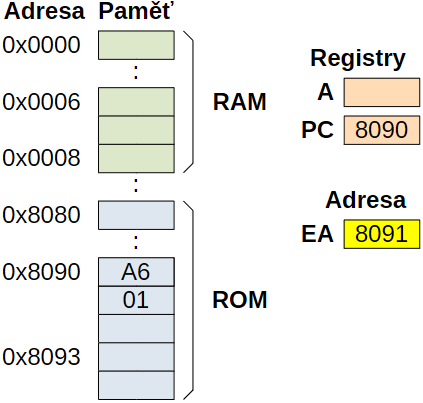
\includegraphics[width=0.45\textwidth]{fig/model_adresace.png} & 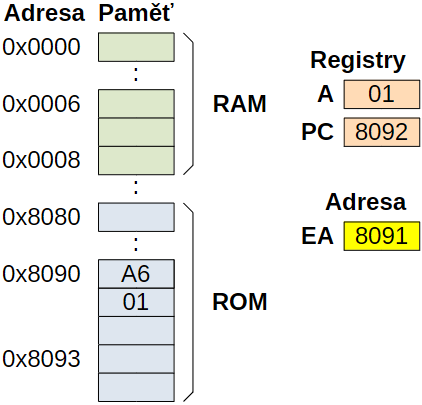
\includegraphics[width=0.45\textwidth]{fig/model_adresace_po.png} \\
				
			\end{tabular}
		\end{center}

	\end{frame}
	
% =====================================================================================================================
	\begin{frame}
    \frametitle{Bezprostřední adresace}
		
		\textbf{Příklad:} \textcolor{blue}{\textbf{LD}} A, \#\$01
		\small
		\begin{center}
			\begin{tabular}{c | c}
				\textbf{Před výkonem instrukce} & \textbf{Po vykonání instrukce} \\ \\
				
				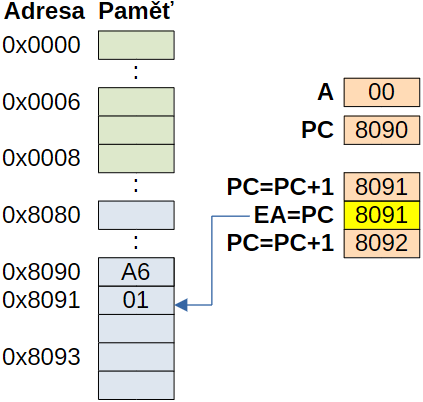
\includegraphics[width=0.45\textwidth]{fig/bezprostredni_adresace.png} & 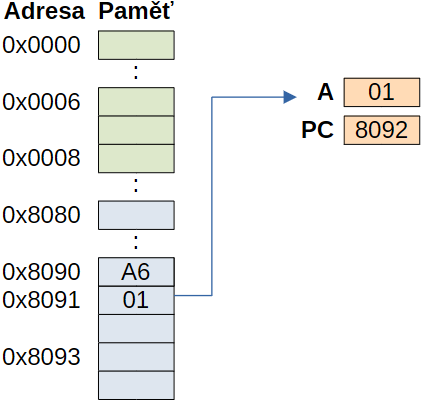
\includegraphics[width=0.45\textwidth]{fig/bezprostredni_adresace_po.png} \\
				
			\end{tabular}
		\end{center}

	\end{frame}
	
% =====================================================================================================================
	\begin{frame}
    \frametitle{Přímá adresace - krátká adresa}
		
		\textbf{Příklad:} \textcolor{blue}{\textbf{LD}} A, \$02 \textcolor{teal}{; adresa má 1 byte}
		\small
		\begin{center}
			\begin{tabular}{c | c}
				\textbf{Před výkonem instrukce} & \textbf{Po vykonání instrukce} \\ \\
				
				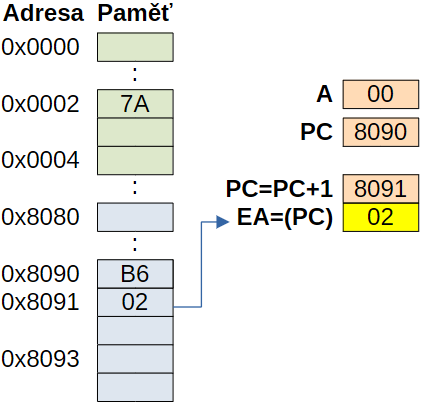
\includegraphics[width=0.45\textwidth]{fig/prima_adresace_K.png} & 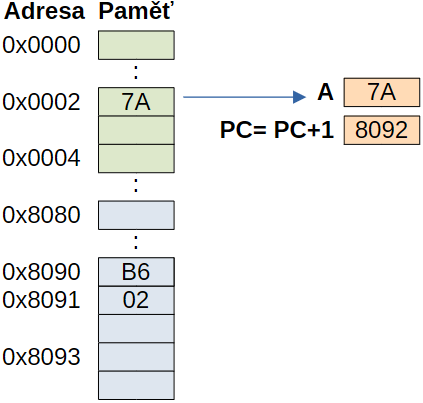
\includegraphics[width=0.45\textwidth]{fig/prima_adresace_K_po.png} \\
				
			\end{tabular}
		\end{center}

		\textbf{Adresace jen v rozsahu 0-255 (0x00 až 0xFF).}
	\end{frame}
	
% =====================================================================================================================
	\begin{frame}
    \frametitle{Přímá adresace - dlouhá adresa}
		
		\textbf{Příklad:} \textcolor{blue}{\textbf{LD}} A, \$100 \textcolor{teal}{; adresa má 2 byte}
		\small
		\begin{center}
			\begin{tabular}{c | c}
				\textbf{Před výkonem instrukce} & \textbf{Po vykonání instrukce} \\ \\
				
				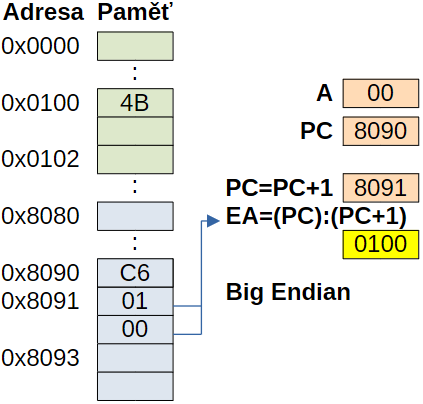
\includegraphics[width=0.45\textwidth]{fig/prima_adresace_D.png} & 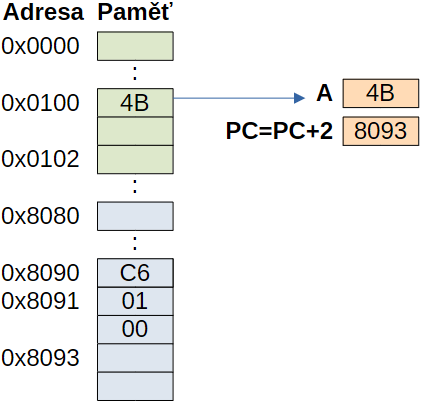
\includegraphics[width=0.45\textwidth]{fig/prima_adresace_D_po.png} \\
				
			\end{tabular}
		\end{center}

		\textbf{Adresace jen v rozsahu 0x0000 až 0xFFFF.}
	\end{frame}
	
% =====================================================================================================================
	\begin{frame}
    \frametitle{Přímá adresace}
		
		\begin{itemize}
			\item Pro instrukce \textcolor{blue}{\textbf{CALLF}} a \textcolor{blue}{\textbf{JPF}} (skoky) se používá ještě rozšířená dlouhá adresace skládající se ze 3 byte:
			
			\begin{itemize}
				\item uložení adresy v paměti v \textbf{Big Endian},
				\item po provedení instrukce se Program Counter zvýší o 3.
			\end{itemize}
			
			\vspace{3mm}
			\item Přímá adresace je používána většinou instrukcí:
			
			\begin{itemize}
				\item čtení z paměti a zapisování do paměti \textcolor{blue}{\textbf{LD}}, \textcolor{blue}{\textbf{MOV}},
				\item logické operace \textcolor{blue}{\textbf{OR}}, \textcolor{blue}{\textbf{XOR}}, ...
				\item aritmetické operace \textcolor{blue}{\textbf{ADD}}, \textcolor{blue}{\textbf{SUB}}, ...
				\item bitové rotace a posuny \textcolor{blue}{\textbf{RLC}}, \textcolor{blue}{\textbf{SLL}}, ...
				\item \textbf{také ji používají absolutní skoky} \textcolor{blue}{\textbf{CALL}}, \textcolor{blue}{\textbf{JP}},
				\item \textbf{a operace ukládání a čtení zásobníku} \textcolor{blue}{\textbf{PUSH}}, \textcolor{blue}{\textbf{POP}}.
			\end{itemize}
			
		\end{itemize}
		
	\end{frame}
	
% =====================================================================================================================
	\begin{frame}
    \frametitle{Indexová adresace}
		
		\begin{itemize}
			\item Používáme pro adresaci polí, tabulek apod.
			\vspace{3mm}
			\item má dvě části:
			
			\begin{itemize}
				\item \textbf{bázi}, která udává počátek adresy a
				\item \textbf{posunutí} nebo také \textbf{offset}, který udává posun (počet kroků, byte) od bázové adresy,
			\end{itemize}
			
			\vspace{3mm}
			\item rozlišujeme:
			
			\begin{itemize}
				\item indexové s nulovým offsetem = nepřímá registrová adresace,
				\item indexové s \textcolor{red}{\textbf{ne}}nulovým offsetem = indexová adresace,
			\end{itemize}
			
			\vspace{3mm}
			\item pro indexovou adresaci (tj. zápis offsetu) se používají indexové registry \textcolor{blue}{\textbf{X}}, \textcolor{blue}{\textbf{Y}}.
			
		\end{itemize}
		
	\end{frame}
	
% =====================================================================================================================
	\begin{frame}
    \frametitle{Indexová adresace s nulovým offsetem}
		
		\textbf{Příklad:} \textcolor{blue}{\textbf{LD}} A, (X) \textcolor{teal}{; báze = 0}
		\small
		\begin{center}
			\begin{tabular}{c | c}
				\textbf{Před výkonem instrukce} & \textbf{Po vykonání instrukce} \\ \\
				
				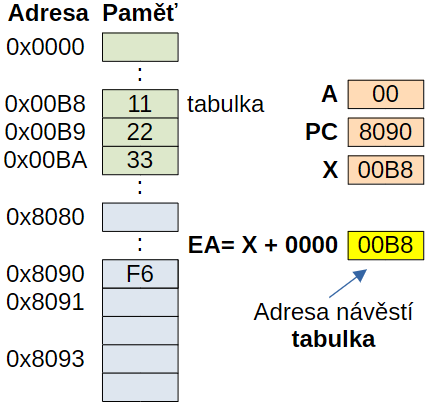
\includegraphics[width=0.45\textwidth]{fig/indexova_adresace_0.png} & 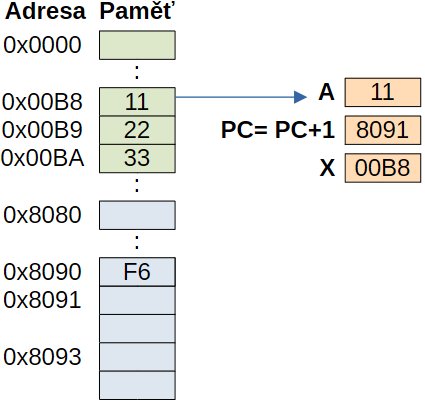
\includegraphics[width=0.45\textwidth]{fig/indexova_adresace_0_po.png} \\
				
			\end{tabular}
		\end{center}

		\textbf{Dovoleno adresovat jen prostor \textcolor{red}{0x00 až 0xFF.}}
	\end{frame}
	
% =====================================================================================================================
	\begin{frame}
    \frametitle{Indexová adresace - krátká adresa}
		
		\textbf{Příklad:} \textcolor{blue}{\textbf{LD}} A, (\$89, X) \textcolor{teal}{; báze = 0x89, posun 2}
		\small
		\begin{center}
			\begin{tabular}{c | c}
				\textbf{Před výkonem instrukce} & \textbf{Po vykonání instrukce} \\ \\
				
				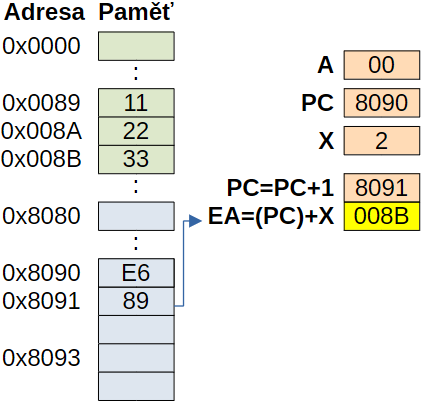
\includegraphics[width=0.45\textwidth]{fig/indexova_adresace_K.png} & 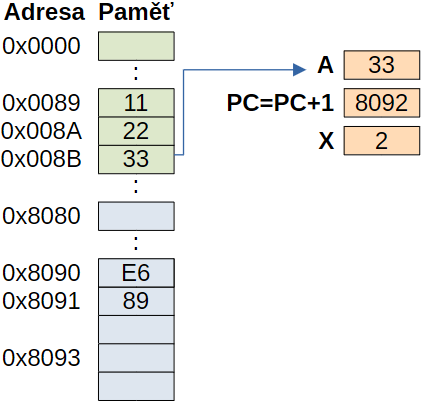
\includegraphics[width=0.45\textwidth]{fig/indexova_adresace_K_po.png} \\
				
			\end{tabular}
		\end{center}

		\textbf{Dovoleno adresovat jen prostor \textcolor{red}{0x00 až 0x1FE.}}
	\end{frame}

% =====================================================================================================================
	\begin{frame}
    \frametitle{Indexová adresace - dlouhá adresa}
		
		\textbf{Příklad:} \textcolor{blue}{\textbf{LD}} A, (\$077E, X) \textcolor{teal}{; báze = 0x077E, posun 1}
		\small
		\begin{center}
			\begin{tabular}{c | c}
				\textbf{Před výkonem instrukce} & \textbf{Po vykonání instrukce} \\ \\
				
				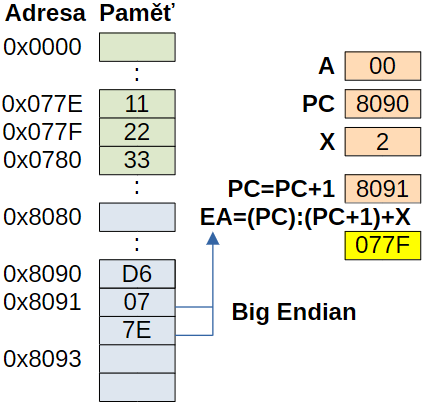
\includegraphics[width=0.45\textwidth]{fig/indexova_adresace_D.png} & 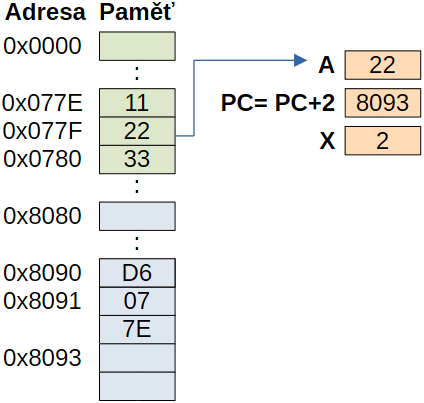
\includegraphics[width=0.45\textwidth]{fig/indexova_adresace_D_po.png} \\
				
			\end{tabular}
		\end{center}

		\textbf{Lze adresovat celý prostor 128 kB.}
	\end{frame}
	
% =====================================================================================================================
	\begin{frame}
    \frametitle{Nepřímá adresace}
		
		\begin{itemize}
			\item \textbf{Adresa dat} je uložena pomocí ukazatele,
			\item \textbf{ukazatel} je jiné paměťové místo, které obsahuje cílovou adresu dat, tj.
				\begin{enumerate}
					\item na adrese ukazatele je přečtena hodnota,
					\item tato hodnota je použita jako adresa pro čtení dat.
				\end{enumerate}
				
			\vspace{3mm}
			\item opět existují varianty:
			
			\begin{itemize}
				\item nepřímé adresování s krátkým nebo dlouhým ukazatelem:
				
				\begin{itemize}
					\item \textcolor{blue}{\textbf{LD}} A, [\$40.w]
					\item \textcolor{blue}{\textbf{LD}} A, [\$1040.w]
				\end{itemize}
				
				\item nepřímé adresování indexové s krátkým neo dlouhým ukazatelem:
				\begin{itemize}
					\item \textcolor{blue}{\textbf{LD}} A, ([\$40.w], X)
					\item \textcolor{blue}{\textbf{LD}} A, ([\$1040.w], X)
				\end{itemize}
			\end{itemize}
			
			\vspace{3mm}
			\item \textbf{z \uv{ukazované} pozice čteme dlouhou adresu $\Rightarrow$ adresujeme celý prostor 64 kB.}
		\end{itemize}
		
	\end{frame}
	
% =====================================================================================================================
	\begin{frame}
    \frametitle{Nepřímá adresace - krátký ukazatel}
		
		\textbf{Příklad:} \textcolor{blue}{\textbf{LD}} A, [\$40.w] \textcolor{teal}
		\small
		\begin{center}
			\begin{tabular}{c | c}
				\textbf{Před výkonem instrukce} & \textbf{Po vykonání instrukce} \\ \\
				
				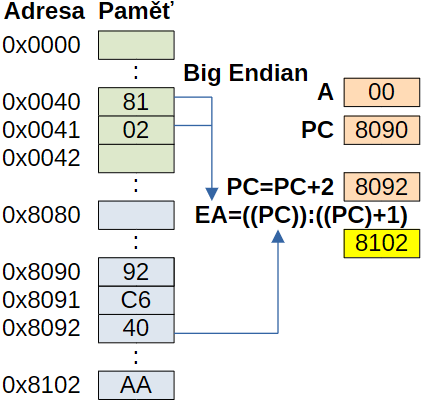
\includegraphics[width=0.45\textwidth]{fig/neprima_adresace_K.png} & 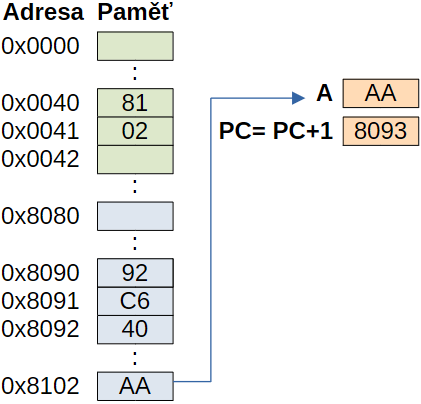
\includegraphics[width=0.45\textwidth]{fig/neprima_adresace_K_po.png} \\
				
			\end{tabular}
		\end{center}

	\end{frame}